\chapter{Software}
\label{chap:software}

The third chapter of this thesis describes the web application, CryptoShow, which is developed to provide a user-friendly interface for the methodology described in Chapter~\ref{chap:methodology}. This chapter covers the architecture, technologies used, backend and frontend development, testing, monitoring, and deployment of the application.

\section{Architecture and Used Technologies}
\label{sec:architecture-technologies}

This section outlines the architecture of the CryptoShow application and the technologies employed in its development. The application is designed to be modular and scalable, allowing for easy integration of new features and improvements. For this purpose, we have chosen a service-oritented architecture (SOA) that separates the components, enabling independent development and deployment. The architecture is defined by several Docker containers, each responsible for a specific part of the application. The services are orchestrated using Docker Compose, defined in the \texttt{docker-compose.yml} file, which specifies the services, networks, and volumes required for the application to run. The service architecture is as follows:

\begin{itemize}
    \item \textbf{backend} - Acts as the central API service, facilitating communication between most components. It communicates with Redis, manages API requests from the frontend, and delegates asynchronous tasks to Celery workers. The FastAPI server serves as its entry point. Further details are provided in Section~\ref{sec:backend}.
    \item \textbf{worker-cpu / worker-gpu} - These two services execute asynchronous, resource-intensive tasks without blocking the main FastAPI event loop. \texttt{worker-cpu} runs on the CPU, while \texttt{worker-gpu} leverages GPU acceleration via CUDA when available.
    \item \textbf{frontend} - Delivers the user interface. NginX acts as the gateway to the defined services in Docker Compose and serves static content from a specified directory. Additional information is available in Section~\ref{sec:frontend}.
    \item \textbf{redis} - Functions as the message broker for Celery workers, enabling efficient task distribution.
    \item \textbf{monitoring-flag} - A lightweight service that creates a flag file to enable the monitoring proxy endpoint.
    \item \textbf{remove-monitoring-flag} - A lightweight service that removes the monitoring flag file, disabling the monitoring endpoint.
    \item \textbf{flower} - Provides real-time monitoring and statistics for Celery tasks and queues.
    \item \textbf{celery-exporter} - Exposes Celery metrics to Prometheus, similarly to the Flower service.
    \item \textbf{prometheus} - Collects and stores metrics exported from the Celery workers.
    \item \textbf{grafana} - Offers a user-friendly dashboard for visualizing metrics collected by Prometheus.
\end{itemize}

\begin{figure}[htpb]
    \centering
    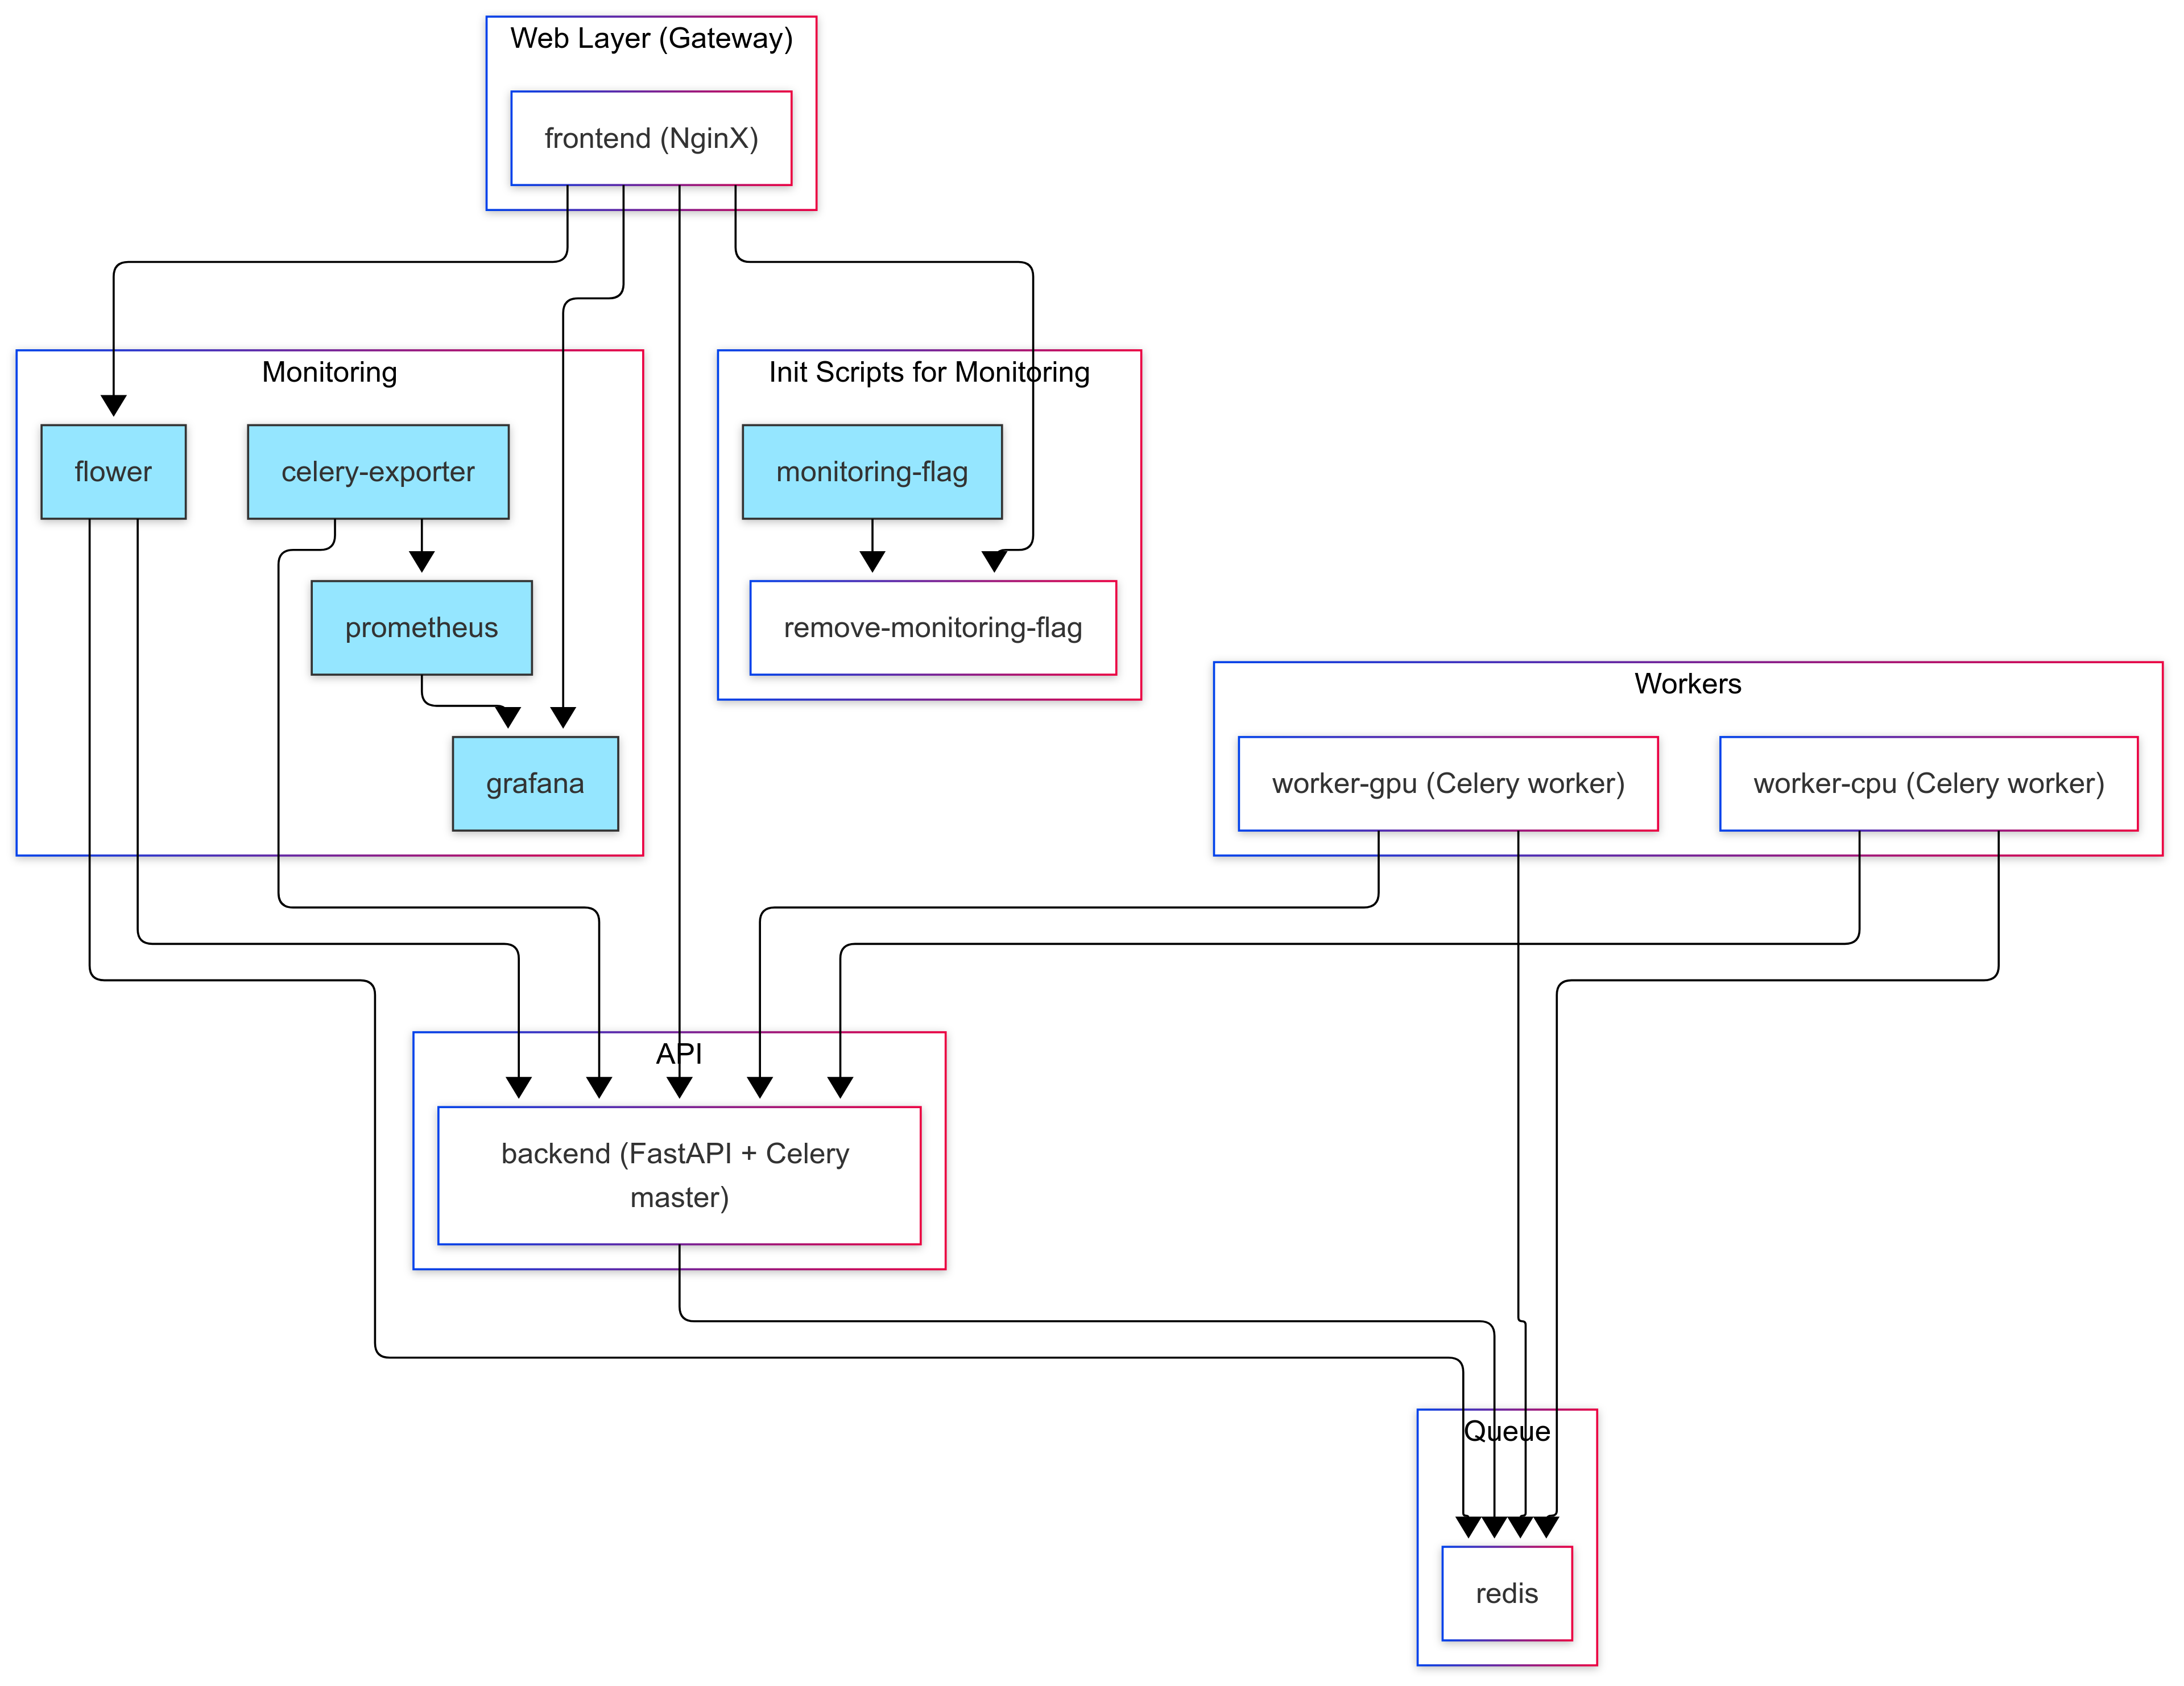
\includegraphics[width=\textwidth]{img/architecture.png}
    \caption{Service architecture of the CryptoShow application. Each box represents a Docker containerized service. Green services are optional, as monitoring is not always required. Arrows indicate communication paths between services. Generated using the Mermaid Live Editor, available at \url{https://mermaid.live/}.}
    \label{fig:architecture}
\end{figure}

An overview of the service architecture can be seen in Figure~\ref{fig:architecture}. This type of architecture offers a scalable solution that has the potential of easy deployment and development.

Let's also focus on the technology stack for some of the services:

\begin{itemize}
    \item \textbf{backend, worker-cpu / worker-gpu} - Python, notable libraries and tools: Celery (asynchronous tasks in Python), FastAPI, Flower, PyTorch, BioPython, Biotite, Scikit-Learn, MDAnalysis, Gemmi, Redis, uv
    \item \textbf{frontend} - TypeScript, notable libraries, tools and frameworks: React, NginX, Mol*, Bun, Vite
\end{itemize}

The remaining services utilize standard technology stacks commonly associated with their respective functionalities.

\section{Backend}
\label{sec:backend}

\xxx{TODO: add the integration of the developed methodology into the backend}
\xxx{TODO: do we include all API endpoints?}

\section{Frontend}
\label{sec:frontend}

\xxx{TODO: describe both frontend overall and the Mol* specifics}


\section{Tests and Monitoring}
\label{sec:tests-monitoring}

\xxx{TODO: add information about Docker healthchecks, monitoring options}


\section{Deployment}
\label{sec:deployment}

\xxx{TODO: describe options for Docker, mention open ports, instructions, maybe requirements for the server}
